\documentclass[12pt, psamsfonts]{amsart}

%-------Packages---------
\usepackage{amssymb,amsfonts}
\usepackage{fullpage}
\usepackage{todonotes}
\usepackage{physics}
\usepackage[all,arc]{xy}
\usepackage{enumerate}
\usepackage{mathrsfs}
\usepackage{theoremref}
\usepackage{graphicx}
\usepackage[bookmarks]{hyperref}

%--------Theorem Environments--------
%theoremstyle{plain} --- default
\newtheorem{thm}{Theorem}[section]
\newtheorem{cor}[thm]{Corollary}
\newtheorem{prop}[thm]{Proposition}
\newtheorem{lem}[thm]{Lemma}
\newtheorem{conj}[thm]{Conjecture}
\newtheorem{quest}[thm]{Question}

\theoremstyle{definition}
\newtheorem{defn}[thm]{Definition}
\newtheorem{defns}[thm]{Definitions}
\newtheorem{con}[thm]{Construction}
\newtheorem{exmp}[thm]{Example}
\newtheorem{exmps}[thm]{Examples}
\newtheorem{notn}[thm]{Notation}
\newtheorem{notns}[thm]{Notations}
\newtheorem{addm}[thm]{Addendum}
\newtheorem*{exer}{Exercise}

\theoremstyle{remark}
\newtheorem{rem}[thm]{Remark}
\newtheorem{rems}[thm]{Remarks}
\newtheorem{warn}[thm]{Warning}
\newtheorem{sch}[thm]{Scholium}

\DeclareMathOperator{\Hom}{Hom}
\DeclareMathOperator{\Id}{Id}

\makeatletter
\let\c@equation\c@thm
\makeatother
\numberwithin{equation}{section}

\bibliographystyle{plain}

\begin{document}

\title{Math 611 Homework (Due 9/25)}
\author{Hidenori Shinohara}
\maketitle

\begin{exer}{(Problem 4, Chapter 1.3)}
  Construct a simply-connected covering space of the space $X \subset \mathbb{R}^3$ that is the union of a sphere and a diameter.
  Do the same when $X$ is the union of a sphere and a circle intersecting it in two points.
\end{exer}

\begin{proof}
  \begin{figure}
    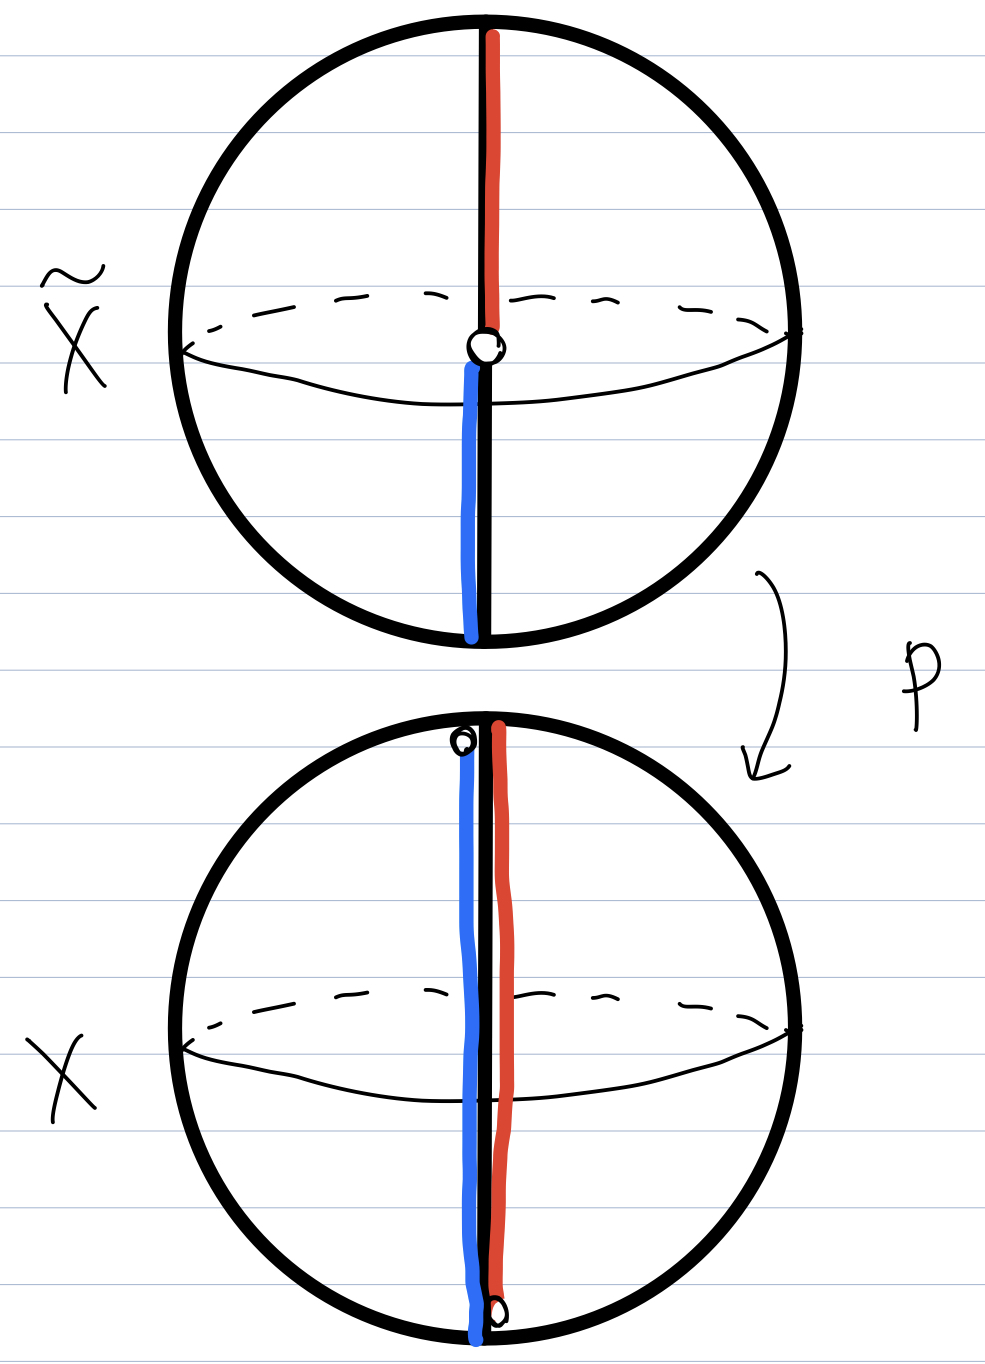
\includegraphics[width=.5\linewidth]{problem4-1.jpeg}
    \caption{Problem 4 (Part 1)}
    \label{fig:prob4_1}
  \end{figure}
  We claim that $\title{X} = X \setminus \{ 0 \}$ is a simply-connected covering space of $X$.
  (See Figure \ref{fig:prob4_1}.)
  \begin{itemize}
    \item
      Simply-connected?
      $\tilde{X}$ deformation retracts onto $S^2$.
      By Proposition 1.17, $\pi_1(\tilde{X}) = \pi_1(S^2)$.
      Proposition 1.14 shows that $\pi_1(S^2) = 0$.
      Therefore, $\tilde{X}$ is simply connected.
    \item
      Covering space?
      Let $p: \tilde{X} \rightarrow X$ be defined such that
      \begin{itemize}
        \item
          $p\mid_{S^2} = \Id_{S^2}$.
          In other words, $p$ maps every point on the spherical part of $\tilde{X}$ to the same place on the spherical part of $X$.
        \item
          $p$ extends the red line to the diameter (the top half of the diameter, in other words, the radius in the northern hemisphere in Figure \ref{fig:prob4_1}).
          In other words, $p$ maps $(0, 1)$ on the $Y$ axis into $(-1, 1)$.
        \item
          $p$ extends the blue line to the diameter (the bottom half of the diameter, in other words, the radius in the southern hemisphere in Figure \ref{fig:prob4_1}).
          In other words, $p$ maps $(-1, 0)$ on the $Y$ axis into $(-1, 1)$.
      \end{itemize}
      Then $p$ is clearly continuous and surjective.
      We will show that every point has a neighborhood that is evenly covered.
      Let $x \in X$ be given.
      \begin{itemize}
        \item
          Case 1: $x$ is on the sphere and is disjoint from the diameter.
          Then a neighborhood of $x$ that is disjoint from the diameter is clearly evenly covered.
        \item
          Case 2: $x$ is on the diameter and is disjoint from the sphere.
          Let $U$ be a neighborhood of $x$ that is disjoint from the sphere.
          Then $U$ is contained in both the image of the red line under $p$ and the image of the blue line under $p$.
          Thus $p^{-1}(U)$ is a union of an open subset of the red line and open subset of the blue line in $\tilde{X}$.
          Therefore, $U$ is evenly covered.
        \item
          Case 3: $x$ is the north pole or south pole.
          \todo[inline]{
            I started to feel like this solution doesn't work because of this case...
          }
      \end{itemize}
  \end{itemize}
\end{proof}

\begin{exer}{(Problem 5, Chapter 1.3)}
  Let $X$ be the subspace of $\mathbb{R}^2$ consisting of the four sides of the square $[0, 1] \times [0, 1]$ together with the segments of the vertical lines $x = 1/2, 1/3, 1/4, \cdots$ inside the square.
  Show that for every covering space $X \rightarrow X$ there is some neighborhood of the left edge of $X$ that lifts homeomorphically to $\tilde{X}$.
  Deduce that $X$ has no simply-connected covering space.
\end{exer}

\begin{proof}
  \todo[inline]{
    Idea:
    Open cover of the left edge by evenly covered open sets.
    Find a finite subcover.
    By the tube lemma, there exists $U \times I$ that covers the left edge and a partition $0 = t_0 < \cdots < t_n = 1$ such that $U \times [t_i, t_{i + 1}]$ is contained in an evenly covered neighborhood.
    Inductively, show $U \times [0, t_i]$ is in an evenly covered neighborhood.
    Lift a loop in $X$ with a vertical line $x = 1/n$ for some large $n$.
    Then the element maps back to itself by $p$.
    In other words, $p_*(\pi_1(\tilde{X})) \ne 0$.
  }
\end{proof}


\end{document}


